\documentclass[tikz,border=2pt]{standalone}
\usepackage{amsmath}
\usepackage{pgfplots}
\pgfplotsset{compat=1.18}
\usetikzlibrary{arrows.meta}
\begin{document}
% f(x) = x^4 - 4x^2 + x on the search interval [-2, 2.5]. optimize(f4, c(-2, 2.5)) returns the
% local minimum x = 1.347, f = -2.619; the global minimum x = -1.473, f = -5.444 is missed.
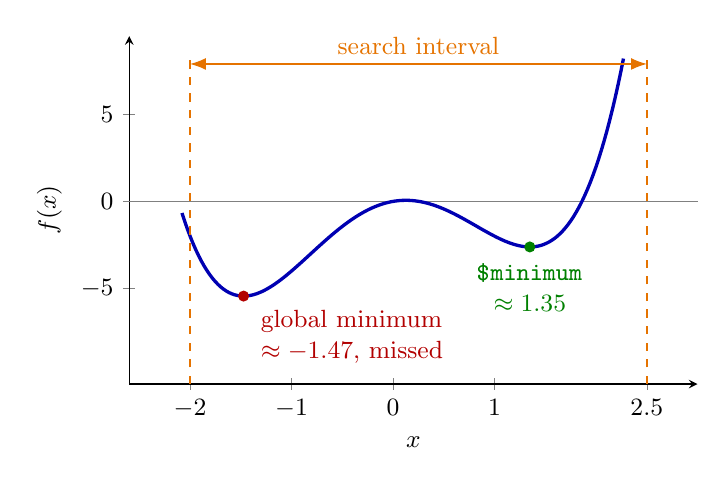
\begin{tikzpicture}[font=\small, >={Latex[length=2mm]}]
  \begin{axis}[width=8.8cm, height=6cm, axis lines=left, xmin=-2.6, xmax=3.0, ymin=-10.5, ymax=9.5,
      xtick={-2,-1,0,1,2.5}, ytick={-5,0,5}, xlabel={$x$}, ylabel={$f(x)$},
      tick label style={font=\small}, label style={font=\small}, clip=false]
    \draw[gray, thin] (axis cs:-2.6,0) -- (axis cs:3.0,0);
    \addplot[blue!70!black, very thick, domain=-2.08:2.27, samples=161] {x^4-4*x^2+x};
    \draw[orange!90!black, dashed, thick] (axis cs:-2,-10.5) -- (axis cs:-2,8.2);
    \draw[orange!90!black, dashed, thick] (axis cs:2.5,-10.5) -- (axis cs:2.5,8.2);
    \draw[orange!90!black, <->] (axis cs:-2,7.9) -- node[above] {search interval} (axis cs:2.5,7.9);
    \fill[green!50!black] (axis cs:1.347,-2.619) circle (2pt);
    \node[green!50!black, anchor=north, align=center] at (axis cs:1.347,-3.0) {\texttt{\$minimum}\\$\approx1.35$};
    \fill[red!70!black] (axis cs:-1.473,-5.444) circle (2pt);
    \node[red!70!black, anchor=north west, align=left] at (axis cs:-1.40,-5.7) {global minimum\\$\approx-1.47$, missed};
  \end{axis}
\end{tikzpicture}
\end{document}
